\part{Permissões}

% ------------------------------------------------------------------------
\chapter{Grupos, Usuários, Poderes e Permissões}\label{chap:permissoes}
% ------------------------------------------------------------------------
\begin{figure}[h!]
    \centering
    \includegraphics[width=0.8\textwidth]{imgs/linux_permissions.png}
    \caption{Visão geral de usuários, grupos e permissões no Linux.}
\end{figure}

O Linux é um sistema multiusuário que controla o acesso através de UIDs (User IDs) e GIDs (Group IDs) \cite{love:linuxkernel,tanenbaum:mos}.

\section{Gerenciamento de Usuários e Grupos}\label{sec:usuarios-grupos}
\begin{itemize}
    \item \textbf{Arquivos de Configuração:}
    \begin{itemize}
        \item \texttt{/etc/passwd}: Mapeia usuários para UIDs, shells e diretórios home.
        \item \texttt{/etc/shadow}: Armazena as senhas criptografadas (hashes) de forma segura.
        \item \texttt{/etc/group}: Define os grupos e seus membros.
    \end{itemize}
    \item \textbf{Comandos:} \texttt{adduser}, \texttt{deluser}, \texttt{passwd}, \texttt{addgroup}.
\end{itemize}

\begin{figure}[h!]
    \centering
    \includegraphics[width=0.8\textwidth]{imgs/user_data.png}
    \caption{Propriedades do usuário no Linux.}
\end{figure}

\section{Permissões de Arquivos (Modo Octal e Simbólico)}\label{sec:permissoes-arquivos}
Cada arquivo possui permissões para Dono (u), Grupo (g) e Outros (o) \cite{silberschatz:osc}. A estrutura de metadados de cada arquivo (inode) é detalhada no Capítulo \ref{chap:filesystem}.
\begin{itemize}
    \item \textbf{Tipos:} Leitura (\textbf{r}=4), Escrita (\textbf{w}=2), Execução (\textbf{x}=1).
    \item \textbf{Comandos:}
    \begin{itemize}
        \item \texttt{chmod}: Altera as permissões (ex: \texttt{chmod 755 arquivo}).\footnote{Manual: \url{https://man7.org/linux/man-pages/man1/chmod.1.html}}
        \item \texttt{chown}: Altera o dono e o grupo (ex: \texttt{chown user:group arquivo}).\footnote{Manual: \url{https://man7.org/linux/man-pages/man1/chown.1.html}}
    \end{itemize}
\end{itemize}

\section{Privilégios Especiais}\label{sec:privilegios-especiais}
O usuário \texttt{root} (UID 0) tem acesso total. O comando \texttt{sudo} (\textit{SuperUser Do}) permite que usuários comuns executem comandos com privilégios elevados, configurados via \texttt{/etc/sudoers} \cite{stallings:os}. Essa elevação é frequentemente necessária para operações de montagem de partições (ver Capítulo \ref{chap:particoes}).

% ------------------------------------------------------------------------
\chapter{Gerenciamento de Processos}\label{chap:processos}
% ------------------------------------------------------------------------
Um processo é uma instância de um programa em execução. O gerenciamento de processos é central para o sistema operacional, permitindo multitarefa através de \textit{time sharing} \cite{tanenbaum:mos,silberschatz:osc}. Processos essenciais são disparados já na fase de inicialização (Capítulo \ref{chap:boot}).

\section{Identificação e Estrutura}\label{sec:identificacao-processo}
\begin{itemize}
    \item \textbf{PID:} Todo processo possui um identificador único (\textit{Process ID}).
    \item \textbf{PCB (Process Control Block):} Estrutura de dados no Kernel que armazena o contexto do processo (registradores, estado, prioridade, contadores).
    \item \textbf{Contexto:} Hardware (registradores da CPU), Software (quotas, privilégios) e Endereçamento (memória alocada).
\end{itemize}

\section{Estados do Processo}\label{sec:estados-processo}
Um processo transita entre estados:
\begin{enumerate}
    \item \textbf{Execução (Running):} Está usando a CPU.
    \item \textbf{Pronto (Ready):} Aguardando vez na CPU (escalonamento).
    \item \textbf{Espera (Wait/Blocked):} Aguardando um evento (ex: E/S).
\end{enumerate}
A troca entre processos é chamada de \textit{Mudança de Contexto} \cite{love:linuxkernel}.

\begin{table}[h!]
    \centering
    \begin{adjustbox}{width=\textwidth}
        \begin{tabular}{|l|l|l|}
            \hline
            \textbf{Estado} & \textbf{Descrição resumida}   & \textbf{Referência}     \\
            \hline
            Running       & Em execução na CPU            & \cite{tanenbaum:mos}    \\
            Ready         & Apto, aguardando CPU          & \cite{silberschatz:osc} \\
            Blocked       & Esperando evento E/S          & \cite{stallings:os}     \\
            Zombie        & Finalizado, aguardando coleta & \cite{love:linuxkernel} \\
            Stopped       & Suspenso por sinal            & \cite{love:linuxkernel} \\
            \hline
        \end{tabular}
    \end{adjustbox}
    \caption{Estados de processo e descrição.}\label{tab:estados-processo}
\end{table}

\section{Monitoramento}\label{sec:monitoramento-processo}
O sistema de arquivos virtual \texttt{/proc} expõe informações do Kernel sobre processos. Comandos como \texttt{top}, \texttt{htop}, \texttt{ps} e \texttt{uptime} (para ver média de carga/load average) são usados para monitoramento \cite{love:linuxkernel}. A interação com \texttt{/proc} complementa a análise de desempenho de discos (Capítulo \ref{chap:memoria-secundaria}).\footnote{Documentação: \url{https://man7.org/linux/man-pages/man5/proc.5.html}}

% ------------------------------------------------------------------------
\chapter{Gerenciamento de Memória Primária}\label{chap:memoria}
% ------------------------------------------------------------------------
O gerenciador de memória controla o acesso da CPU à memória principal (RAM), alocando e desalocando espaços para processos.

\section{Tipos de Memória}\label{sec:tipos-memoria}
\begin{itemize}
    \item \textbf{RAM (Random Access Memory):} Memória volátil de acesso rápido. Divide-se em DRAM (Dinâmica, precisa de refresh, usada na memória principal) e SRAM (Estática, mais rápida, usada em Cache L1/L2).
    \item \textbf{Cache:} Armazena dados usados frequentemente para reduzir o tempo de acesso à DRAM.
\end{itemize}

\begin{figure}[h!]
    \centering
    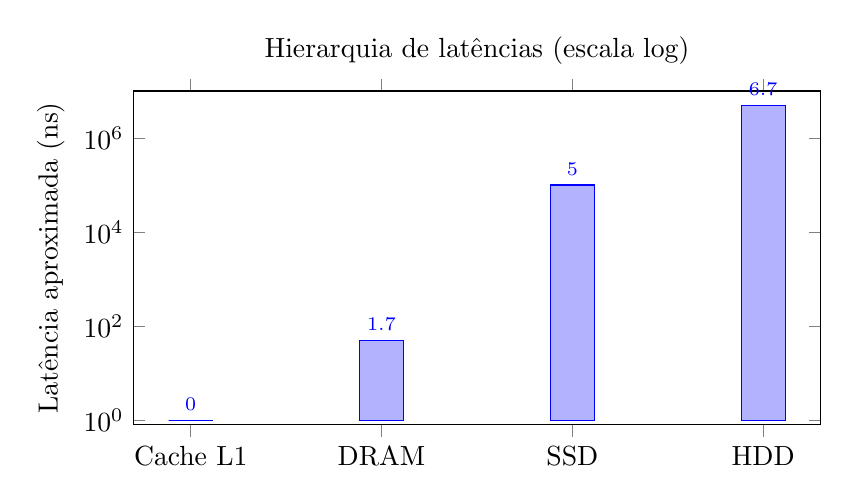
\begin{tikzpicture}
        \begin{axis}[
            ybar,
            width=0.85\textwidth,
            height=0.48\textwidth,
            bar width=16pt,
            ylabel={Latência aproximada (ns)},
            symbolic x coords={Cache L1,DRAM,SSD,HDD},
            xtick=data,
            ymode=log,
            log basis y={10},
            ymin=0.8,
            ymax=10000000,
            nodes near coords,
            nodes near coords align={vertical},
            every node near coord/.append style={font=\scriptsize},
            title={Hierarquia de latências (escala log)}
        ]
            \addplot coordinates {(Cache L1,1) (DRAM,50) (SSD,100000) (HDD,5000000)};
        \end{axis}
    \end{tikzpicture}
    \caption{Ordem de grandeza de latências de memória e armazenamento.}\label{fig:latencias-hierarquia}
\end{figure}

\noindent Valores ilustrativos baseados em ordens de grandeza.\footnote{Referência de latências: \url{https://people.eecs.berkeley.edu/~rcs/research/interactive_latency.html}} Ver Capítulo \ref{chap:memoria-secundaria} para detalhes físicos de SSD e HDD \cite{patterson:hennessy}.

\section{Técnicas de Gerenciamento}\label{sec:tecnicas-gerenciamento}
\begin{itemize}
    \item \textbf{Endereçamento Virtual:} Os processos usam endereços lógicos que são traduzidos para endereços físicos pela MMU (Memory Management Unit). Isso isola a memória de cada processo \cite{tanenbaum:mos,silberschatz:osc}.
    \item \textbf{Paginação:} Divide a memória em blocos de tamanho fixo chamados páginas (geralmente 4KB). Permite carregar partes do processo sob demanda e elimina fragmentação externa \cite{stallings:os}.
    \item \textbf{Segmentação:} Divide a memória em segmentos de tamanhos variáveis baseados na lógica do programa (código, dados, pilha) \cite{silberschatz:osc}.
    \item \textbf{Swapping:} Quando a RAM está cheia, o sistema move processos inativos para uma área no disco (Swap), liberando memória principal. O acesso ao disco é significativamente mais lento que à RAM \cite{patterson:hennessy}.
\end{itemize}

\begin{table}[h!]
    \centering
    \begin{adjustbox}{width=\textwidth}
        \centering
        \begin{tabular}{|l|l|l|l|}
            \hline
            \textbf{Permissão} & \textbf{Valor} & \textbf{Descrição}           & \textbf{Referência}     \\
            \hline
            r                & 4              & Leitura                      & \cite{silberschatz:osc} \\
            w                & 2              & Escrita                      & \cite{stallings:os}     \\
            x                & 1              & Execução                     & \cite{love:linuxkernel} \\
            rwx              & 7              & Leitura + Escrita + Execução & \cite{tanenbaum:mos}    \\
            rw-              & 6              & Leitura + Escrita            & (POSIX)                 \\
            r-x              & 5              & Leitura + Execução           & (POSIX)                 \\
            ---              & 0              & Sem acesso                   & (POSIX)                 \\
            \hline
        \end{tabular}
    \end{adjustbox}
    \caption{Mapa de permissões simbólicas e octais.}\label{tab:permissoes-octal}
\end{table}